\documentclass[table]{beamer}

\usepackage{kotex}
\usepackage{amsmath}
\usepackage{amssymb}
\usepackage{verbatim}
\ifxetex
 \setsansfont{TeX Gyre Heros}
 \setsanshangulfont{맑은 고딕}
\fi
\usepackage{color, colortbl}					%tabular에서 rowcolor를 변경하기 위해서..
\usepackage{fancybox}
\usepackage{graphbox,graphicx}
\usepackage{tikz}								%오버레이에 그림을 그리기 위해서..
\usepackage{hyperref}							%하이퍼링크 처리

\usepackage{array}
\usepackage{ebproof}
\usepackage{multirow}


\usepackage{xcolor,multirow}
\usepackage{hhline}

\usepackage[T1]{fontenc}
\usepackage{textcomp}
\usepackage{listings}							%자바 코드를 위해서..
\lstset{
	mathescape,
	language=Java,
	basicstyle=\footnotesize\ttfamily,
	keywordstyle={}, % \footnotesize\color{blue}\ttfamily,
	captionpos=b,
	escapeinside=@@,
	showstringspaces=false,					%공백 문제 제거를 위해서
	tabsize=2,
	upquote=true
}

%----------------- 총 페이지수에서 백업 슬라이드를 제거하기 위해서....
\newcommand{\backupbegin}{
   \newcounter{framenumberappendix}
   \setcounter{framenumberappendix}{\value{framenumber}}
}
\newcommand{\backupend}{
   \addtocounter{framenumberappendix}{-\value{framenumber}}
   \addtocounter{framenumber}{\value{framenumberappendix}} 
}
%-----------------

%---------------- tabular에서 rowcolor를 변경하기 위해서..
\definecolor{Gray}{gray}{0.9}
%-----------------

%\usetheme{CambridgeUS}
% \usecolortheme{default}

\usetheme{default}
\usecolortheme{default}

%\usetheme{default}
%\usecolortheme{beaver}
%\usetheme{CambridgeUS}
%\usecolortheme{seagull}

%\useinnertheme{rectangles}


\setbeamertemplate{caption}{\insertcaption}	%그림의 캡션 자동 만들지 않도록.

\addtobeamertemplate{navigation symbols}{}{%
    \usebeamerfont{footline}%
    \usebeamercolor[fg]{footline}%
    \hspace{1em}%
    \insertframenumber/\inserttotalframenumber
}

\title[Types and Programming Languages]{8. Typed Arithmetic Expressions \\
(Types and Programming Languages)}
\author[K. Choi]{Kwanghoon Choi}
\institute[Chonnam National University]{
Software Languages and Systems Laboratory \\
	Chonnam National University}
\date{Week 4}

%%%%% Macros %%%%%

\newcommand{\rpc}{$\lambda_{rpc}$}
\newcommand{\polyrpc}{$\lambda_{rpc}^{\forall}$}
\newcommand{\stateencrpc}{$\lambda_{rpc}^{enc}$}
\newcommand{\statefulrpc}{$\lambda_{rpc}^{state}$}

\newcommand{\cs}{$\lambda_{cs}$}
\newcommand{\stateenccs}{$\lambda_{cs}^{enc}$}
\newcommand{\statefulcs}{$\lambda_{cs}^{state}$}

\newcommand{\client}{\textbf{c}}
\newcommand{\server}{\textbf{s}}
\newcommand{\clientserver}{\textbf{cs}}

\newcommand{\Loc}{Loc}

\newcommand{\evalRPC}[3]{#1\Downarrow_{#2}#3}
\newcommand{\evalRPCC}[2]{#1\Downarrow_{\client}#2}
\newcommand{\evalRPCS}[2]{#1\Downarrow_{\server}#2}
\newcommand{\lamL}[3]{\lambda^{#1}#2.#3}
\newcommand{\appL}[3]{#1{\ }^{#2}#3} 
\newcommand{\subst}[2]{\{#1/#2\}}
\newcommand{\llet}[3]{\textsf{let} \ #1 = #2 \ \textsf{in} \ #3}

\newcommand{\textsfReq}{\textsf{req}}
\newcommand{\req}[2]{\textsfReq(#1,#2)}
\newcommand{\reqwith}[3]{\textsfReq_{#1}(#2,#3)}

\newcommand{\textsfCall}{\textsf{call}}
\newcommand{\call}[2]{\textsfCall(#1,#2)}
\newcommand{\callwith}[3]{\textsfCall_{#1}(#2,#3)}

\newcommand{\textsfRet}{\textsf{ret}}
\newcommand{\ret}[1]{\textsfRet(#1)}
\newcommand{\retwith}[2]{\textsfRet_{#1}(#2)}

\newcommand{\funL}[1]{\xrightarrow{#1}}    
\newcommand{\funLC}[2]{\xrightarrow[#2]{#1}}  
\newcommand{\tyenv}{\Gamma}     
\newcommand{\tyenvExt}[2]{\Gamma\{#1:#2\}}
\newcommand{\tyenvExtWith}[1]{\Gamma,#1}
% \newcommand{\typing}[4]{#1\rhd_{#2} #3 : #4}       
\newcommand{\typing}[4]{#1\vdash_{#2} #3 : #4}       
\newcommand{\typingBlack}[4]{#1\blacktriangleright_{#2} #3 : #4}  

\newcommand{\loceta}[2]{{#1}\rightsquigarrow{#2}}                                         

\newcommand{\enc}{\textsf{enc}}
\newcommand{\evalStateEncRPCC}[2]{$#1\Downarrow_{\client}^{\enc}#2$}
\newcommand{\evalStateEncRPCS}[3]{$#1;#2\Downarrow_{\server}^{\enc}#3$}

\newcommand{\sta}{\textsf{state}}
\newcommand{\evalStatefulRPCC}[3]{\evalStatefulRPC{#1}{#2}{\client}{#3}}
\newcommand{\evalStatefulRPCS}[3]{\evalStatefulRPC{#1}{#2}{\server}{#3}}
\newcommand{\evalStatefulRPC}[4]{${#1};{#2}\Downarrow_{#3}^{\sta}{#4}$}

\newcommand{\deep}{\textsf{deep}}
\newcommand{\evalDeeplyStatefulRPCC}[3]{\evalDeeplyStatefulRPC{#1}{#2}{\client}{#3}}
\newcommand{\evalDeeplyStatefulRPCS}[3]{\evalDeeplyStatefulRPC{#1}{#2}{\server}{#3}}
\newcommand{\evalDeeplyStatefulRPC}[4]{${#1};{#2}\Downarrow_{#3}^{\deep}{#4}$}

\newcommand{\IdK}{\textsf{Id}}
\newcommand{\FunK}[3]{\textsf{Fun} \ #2 \ #3}
\newcommand{\AppK}[3]{\textsf{App} \ #2 \ #3}
%\newcommand{\FunK}[3]{\textsf{Fun}^{#1} \ #2 \ #3}
%\newcommand{\AppK}[3]{\textsf{App}^{#1} \ #2 \ #3}
                                                
\newcommand{\reify}[1]{\ulcorner #1 \urcorner}

\newcommand{\RightarrowEnc}{\Rightarrow^{enc}}
\newcommand{\RightarrowEncStar}{\Rightarrow^{enc*}}
\newcommand{\RightarrowEncPlus}{\Rightarrow^{enc+}}

\newcommand{\runStateEncRPC}[2]{$#1 \RightarrowEnc #2$}
\newcommand{\runStateEncRPCStar}[2]{$#1 \RightarrowEncStar #2$}
\newcommand{\runStateEncRPCPlus}[2]{$#1 \RightarrowEncPlus #2$}

\newcommand{\runStateEncCS}[2]{$#1 \Rightarrow^{enc} #2$}
\newcommand{\runStateEncCSStar}[2]{$#1 \Rightarrow^{enc*} #2$}

\newcommand{\runStatefulRPC}[2]{$#1 \Rightarrow^{state} #2$}
\newcommand{\runStatefulRPCStar}[2]{$#1 \Rightarrow^{state*} #2$}

\newcommand{\runStatefulCS}[2]{$#1 \Rightarrow^{state} #2$}
\newcommand{\runStatefulCSStar}[2]{$#1 \Rightarrow^{state*} #2$}

\newcommand{\emp}{\epsilon}
\newcommand{\substzsxs}{\{\bar{v}/\bar{z},\overline{w}/\bar{x} \}}
\newcommand{\substxs}{\{\overline{w}/\bar{x} \}}

\newcommand{\substZsXs}{\{\overline{V}/\bar{z},\overline{W}/\bar{x} \}}
\newcommand{\substXs}{\{\overline{W}/\bar{x} \}}

\newcommand{\LetK}[2]{\textsf{ctx}\ #1 \ #2}
%\newcommand{\LetK}[2]{(#1,#2)}
\newcommand{\opt}[1]{#1_{opt}}

\newcommand{\overlineK}{\overline{K}}
\newcommand{\overlinePi}{\overline{\Pi}}
\newcommand{\overlineDelta}{\overline{\Delta}}

%\newcommand{\comp}[1]{\rightsquigarrow_{#1}}
%\newcommand{\comps}{\rightsquigarrow_{\server}}
%\newcommand{\compc}{\rightsquigarrow_{\client}}
\newcommand{\ccomp}[1]{C[\![#1]\!]}
\newcommand{\scomp}[1]{S[\![#1]\!]}
\newcommand{\vcomp}[1]{V[\![#1]\!]}
\newcommand{\cconv}[1]{CC[\![#1]\!]}
%\newcommand{\cconvprg}[1]{CC_{prg}[\![#1]\!]}

\newcommand{\FUNS}{\Phi}
\newcommand{\fv}[1]{\textsf{fv}(#1)}
\newcommand{\dom}[1]{\textsf{dom}(#1)}
\newcommand{\clo}[2]{clo({#1},{#2})}

\newcommand{\sessionNothing}{\makebox[0.3cm][c]{\scriptsize $nothing$}}
\newcommand{\sessionSomething}{\makebox[0.3cm][c]{\scriptsize $session$}}
\newcommand{\sessionOption}{\makebox[0.3cm][c]{\scriptsize $optSession$}}

\newcommand{\mono}[1]{[\![#1]\!]}

\newcommand{\eqdef}{\overset{\mathrm{def}}{=\joinrel=}}

%%
%\newtheorem{lemma}{Lemma}[section]
%\newtheorem{theorem}{Theorem}[section]
%\newtheorem{fact}{Fact}[section]
%\newtheorem{definition}{Definition}[section]

%%%%%%%%%%%%%%%%%%

\begin{document}

%\section{Relative Pronoun}
\begin{frame}
%\begin{center}
%{\footnotesize
%Types and Programming Languages
%}
%\end{center}
	\titlepage
	
%	\begin{center}
%	{
%  (Joint work with James Cheney, Simon Fowler, and Sam Lindley)
%	}
%	\end{center}
\end{frame}

%\begin{frame}{Table of Contents}
%\begin{itemize}
%\item
%\item
%\item
%\item
%\end{itemize}
%\end{frame}

%%%
\begin{frame}[t]{A Plan} \vspace{10pt}

Now we augment the arithmetic PL with static types. The type system itself is nearly trivial, but it provides concepts that will recur.

\end{frame}

%%%
\begin{frame}[t]{8.1 Remind: terms, values, and ``stuck''} \vspace{10pt}

Recall the syntax for arithmetic expressions:
\begin{eqnarray*}
\texttt{t} & ::= & \texttt{true} \ | \ 
 \texttt{false} \ | \ 
 \texttt{if} \ \texttt{t} \ \texttt{then} \ \texttt{t} \ \texttt{else} \ t \\
 & | & \texttt{0} \ | \ 
 \texttt{succ t} \ | \ 
 \texttt{pred t} \ | \ 
 \texttt{iszero t} 
\end{eqnarray*}

Evaluating a term can either result in a value 
\begin{eqnarray*}
\texttt{v} & ::= & \texttt{true} \ | \  \texttt{false} \ | \  \texttt{nv} \\
\texttt{nv} & ::= & \texttt{0} \ | \ \texttt{succ nv}
\end{eqnarray*}

or else get {\it stuck}, for example, by reaching a term like \texttt{pred false}.

\vspace{10pt}

Stuck terms correspond to erroneous programs.

\end{frame}

%%%
\begin{frame}[t]{Types} \vspace{10pt}

We would like to be able to tell, without actually evaluating a term, that its evaluation will definitely not get stuck. 

\vspace{10pt}

To do this, we need to be able to distinguish between numeric terms (whose result will be a numeric value) and boolean terms (whose result will be a boolean value).

\vspace{10pt}

We introduce two types for classifying terms in this way. 
\begin{eqnarray*}
Types \ \ \ \texttt{T} & ::= & \texttt{Nat} \ | \  \texttt{Bool} 
\end{eqnarray*}

A term \texttt{t} has type \texttt{T} :
\begin{itemize}
\item \texttt{true : Bool}, \ \ \ \texttt{0 : Nat}.
\item \texttt{if true then false else true} has type \texttt{Bool}.
\item \texttt{pred (succ (pred (succ 0)))} has type \texttt{Nat}.
\end{itemize}

\end{frame}


%%%
\begin{frame}[t]{8.2 The Typing Relation: typing rules or type inference rules}

The typing relation is written as ``\texttt{t : T}'' (a term \texttt{t} has type \texttt{T}). 

\vspace{10pt}

The typing rules
\begin{center}
\begin{tabular}{c l}
\texttt{true : Bool} & (T-True)\\[0.3cm]
\texttt{false : Bool} & (T-False)\\[0.3cm]
\mbox{
\begin{prooftree}
\hypo{ \texttt{t1 : Bool} \ \ \ \ \ \ \texttt{t2 : T} \ \ \ \ \ \ \texttt{t3 : T} }
\infer1[]{ \texttt{if t1 then t2 else t3 : T} }
\end{prooftree}
}
&
(T-IF)\\[0.5cm]
\texttt{0 : Nat} & (T-Zero)\\[0.3cm]
\mbox{
\begin{prooftree}
\hypo{ \texttt{t1 : Nat} }
\infer1[]{ \texttt{succ t1 : Nat} }
\end{prooftree}
}
&
(T-Succ)\\[0.5cm]
\mbox{
\begin{prooftree}
\hypo{ \texttt{t1 : Nat} }
\infer1[]{ \texttt{pred t1 : Nat} }
\end{prooftree}
}
&
(T-Pred)\\[0.5cm]
\mbox{
\begin{prooftree}
\hypo{ \texttt{t1 : Nat} }
\infer1[]{ \texttt{iszero t1 : Bool} }
\end{prooftree}
}
&
(T-IsZero)\\[0.5cm]
\end{tabular}
\end{center}

\end{frame}

%%%
\begin{frame}[t]{The Typing Relation: How to read typing rules} \vspace{10pt}

(1) Axiom \ \ \ \texttt{true : Bool}  

\vspace{10pt}

\begin{itemize}
\item The term \texttt{true} has type \texttt{Bool} {\it unconditionally}. 
\end{itemize}

\vspace{20pt}

(2) Inference rule \ \ \  \mbox{
\begin{prooftree}
\hypo{ \texttt{t1 : Nat} }
\infer1[]{ \texttt{iszero t1 : Bool} }
\end{prooftree}
} 

\vspace{10pt}

\begin{itemize}
\item The term \texttt{iszero t1} has type \texttt{Bool} if \texttt{t1} has type \texttt{Nat}. 
\item ``\texttt{t1 : Nat}'' above the  line is called a condition or a premise, and
\item ``\texttt{iszero t1 : Bool}'' below the  line is called a conclusion.
\end{itemize}


\end{frame}

%%%
\begin{frame}[t]{The Typing Relation: Well-typed terms} \vspace{10pt}

A term \texttt{t} is typeable (or well typed) \\ if there is some \texttt{T} such that \texttt{t: T}.

\vspace{20pt}

Q. \texttt{if true then false else true : ???}

\vspace{10pt}

Q. \texttt{pred (succ (pred (succ 0))) : ???}

\vspace{10pt}

Q. \texttt{if iszero 0 then 0 else pred 0 : ???}

\vspace{10pt}

Q. \texttt{pred false : ???}

\vspace{20pt}

cf. ``A term is typeable'' means that a term can have some type. 

\end{frame}

%%%
\begin{frame}[t]{The Typing Relation: typing derivation} \vspace{10pt}

A typing derivation is a tree of instances of the typing rules. 

\vspace{10pt}

For example,

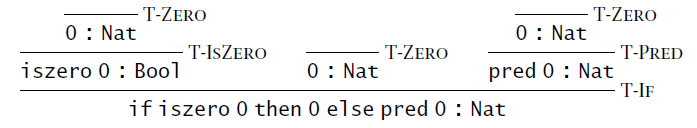
\includegraphics[width=10cm]{typingderivation_ch8}

\end{frame}

%%%
\begin{frame}[t]{The Typing Relation: Some properties} \vspace{10pt}

Lemma 8.2.2 [Inversion of the typing relation]
\begin{itemize}
\item If \texttt{true : T} then \texttt{T = Bool}.
\item If \texttt{false : T} then \texttt{T = Bool}.
\item If \texttt{if t1 then t2 else t3 : T} \\ then \texttt{t1 : Bool}, \texttt{t2 : T}, and \texttt{t3 : T}.
\item If \texttt{0 : T} then ??? % \texttt{T = Nat}.
\item If \texttt{succ t1 : T} then ??? % \texttt{T = Nat} and {t1 : Nat}.
\item If \texttt{pred t1 : T} then ??? % \texttt{T = Nat} and {t1 : Nat}.
\item If \texttt{iszero t1 : T} then ??? % \texttt{T = Bool} and {t1 : Nat}.
\end{itemize}

\vspace{10pt}

Q. Complete the lemma by filling in the holes ???.

\vspace{10pt}

Note that the inversion properityis is not always true for arbitrary type systems but it is true for the one in the arithmetic PL. 

\end{frame}

%%%
\begin{frame}[t]{The Typing Relation: Some properties} \vspace{10pt}

Lemma 8.2.4 [Uniquness of Types] Each term \texttt{t} has at most one type. That is, if \texttt{t} is typable, then its type is unique. 

\vspace{10pt}

Moreover, there is just one derivation of this typing built from the inference rules for the arithmetic expressions.

\vspace{10pt}

Q. Prove the lemma by structural induction on \texttt{t}.

\end{frame}


%%%
\begin{frame}[t]{8.3 Safety = Progress + Preservation} \vspace{10pt}

The most basic property of this type system or any other is {\it safety} (also called {\it soundness}):
\begin{itemize}
\item Well-typed terms do not ``go wrong.''
\end{itemize}

\vspace{10pt}

Terms that went wrong are what evaluate to a term who got stuck.

\vspace{10pt}

What we want to know is that well-typed terms do not get stuck. 

\vspace{10pt}

We show the type safety by proving two steps, commonly known as the {\it progress} and {\it preservation} theorems.

\begin{itemize}
\item Progress: A well-typed term is not stuck (either it is a value or it can take a step according to the evaluation rules).
\item Preservation: If a well-typed term takes a step of evaluation, then the resulting term is also well-typed.
\end{itemize}

\end{frame}

%%%
\begin{frame}[t]{Safety: Progress} \vspace{10pt}

Progress: A well-typed term is not stuck (either it is a value or it can take a step according to the evaluation rules).

\vspace{10pt}

Theorem[Progress] If \texttt{t : T} then 
\begin{itemize}
\item either \texttt{t} is a value 
\item or there is some \texttt{t'} with $\texttt{t}\rightarrow\texttt{t'}$.
\end{itemize}

\vspace{10pt}

Q. Prove this theorem by induction on a derivation of \texttt{t : T}.

\end{frame}

%%%
\begin{frame}[t]{Safety: Preservation} \vspace{10pt}

Preservation: If a well-typed term takes a step of evaluation, then the resulting term is also well-typed.

\vspace{10pt}

Theorem[Preservation] 
If \texttt{t : T} and $\texttt{t}\rightarrow\texttt{t'}$ then \texttt{t' : T}.

\vspace{10pt}

Q. Prove this theorem by induction on a derivation of \texttt{t : T}.

\end{frame}

%%%
\begin{frame}[t]{Summary: The typed arithmetic programming language} \vspace{10pt}

\underline{The syntax of terms and types}

\vspace{10pt}

\begin{tabular}{l c l }
Terms \ \ \ \texttt{t} & $::=$ &
	\texttt{v} \ $|$ \ \texttt{if t then t else t} \\
	& $|$ & \texttt{0} \ $|$ \ \texttt{succ t} \ $|$ \ \texttt{pred t} \ $|$ \ \texttt{iszero t} \\
Values \ \ \  \texttt{v} & $::=$ & \texttt{true} \ $|$ \ \texttt{false} \ $|$ \ \texttt{nv}\\
Num. values \ \texttt{nv} & $::=$ & \texttt{0} \ $|$ \ \texttt{succ nv}
\end{tabular}

\vspace{20pt}

\begin{tabular}{l c l }
Types \ \ \ \texttt{T} & ::= & \texttt{Nat} \ | \  \texttt{Bool} 
\end{tabular}

\end{frame}

%%%
\begin{frame}[t]{Summary: The typed arithmetic PL (cont.)} 

\underline{The (dynamic) semantics}

\begin{center}
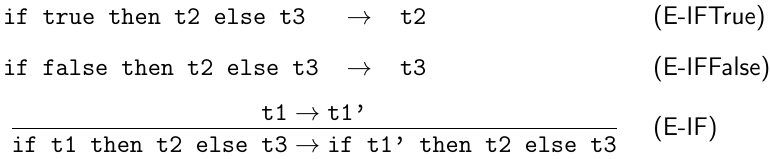
\includegraphics[width=9cm]{evaluation_bool_ch3}
\end{center}

\begin{center}
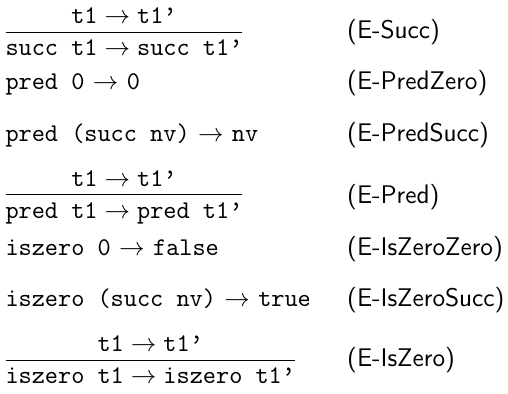
\includegraphics[width=6cm]{evaluation_numeric_ch3}
\end{center}

\end{frame}

%%%
\begin{frame}[t]{Summary: The typed arithmetic PL (cont.)} \vspace{10pt}

\underline{The type system}

\vspace{10pt}

\begin{center}
\begin{tabular}{c l}
\texttt{true : Bool} & (T-True)\\[0.3cm]
\texttt{false : Bool} & (T-False)\\[0.3cm]
\mbox{
\begin{prooftree}
\hypo{ \texttt{t1 : Bool} \ \ \ \texttt{t2 : T} \ \ \ \texttt{t3 : T} }
\infer1[]{ \texttt{if t1 then t2 else t3 : T} }
\end{prooftree}
}
&
(T-IF)\\[0.5cm]
\mbox{
\begin{prooftree}
\hypo{ \texttt{t1 : Nat} }
\infer1[]{ \texttt{succ t1 : Nat} }
\end{prooftree}
}
&
(T-Succ)\\[0.5cm]
\mbox{
\begin{prooftree}
\hypo{ \texttt{t1 : Nat} }
\infer1[]{ \texttt{pred t1 : Nat} }
\end{prooftree}
}
&
(T-Pred)\\[0.5cm]
\mbox{
\begin{prooftree}
\hypo{ \texttt{t1 : Nat} }
\infer1[]{ \texttt{iszero t1 : Bool} }
\end{prooftree}
}
&
(T-IsZero)\\[0.5cm]
\end{tabular}
\end{center}

\end{frame}

%%%
\begin{frame}[t]{Summary: The arithmetic PL - Typing derivations} 

A typing derivation tree for 
\begin{itemize}
\item \texttt{if iszero 0 then 0 else pred 0 : Nat}
\end{itemize}

\vspace{10pt}

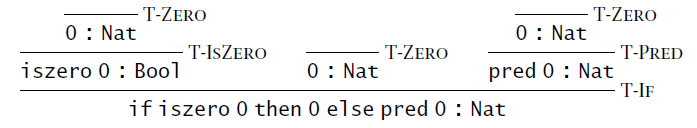
\includegraphics[width=10cm]{typingderivation_ch8}

\end{frame}

%%%
\begin{frame}[t]{Summary: The arithmetic PL - Type safety} 

\underline{Type safety}

\vspace{5pt}

\begin{itemize}
\item If \texttt{t : T} then there is no term \texttt{t'} such that $t \rightarrow^* t'$ and \texttt{t'} is stuck.
\end{itemize}

\vspace{10pt}

A technique to show the type safety is to prove the progress and the preservation properties.
\begin{itemize}
\item Progress: If \texttt{t : T} then either \texttt{t} is a value or there exists a term \texttt{t'} such that $t \rightarrow t'$.
\item Preservation: If \texttt{t : T} and $t \rightarrow t'$ then \texttt{t' : T}.
\end{itemize}



\end{frame}
\end{document}
